\documentclass[12pt]{article}
\usepackage[utf8]{inputenc}
\usepackage{graphicx} % Allows you to insert figures
\usepackage{amsmath} % Allows you to do equations
\usepackage{fancyhdr} % Formats the header
\usepackage{geometry} % Formats the paper size, orientation, and margins
\linespread{1.25} % about 1.5 spacing in Word
\setlength{\parindent}{0pt} % no paragraph indents
\setlength{\parskip}{1em} % paragraphs separated by one line
\usepackage[format=plain,
            font=it]{caption} % Italicizes figure captions
\usepackage[english]{babel}
\usepackage{csquotes}
\renewcommand{\headrulewidth}{0pt}
\geometry{letterpaper, portrait, margin=1in}
\setlength{\headheight}{14.49998pt}

\newcommand\titleofdoc{\textbf{Assignment-4: Fourier Approximations}}
\newcommand\GroupName{EE20B136}

\begin{document}
\begin{titlepage}
   \begin{center}
        \vspace*{4cm} % Adjust spacings to ensure the title page is generally filled with text

        \Huge{\titleofdoc} 

        \vspace{3 cm}
        \Large{Syam SriBalaji T}
       
        \vspace{0.25cm}
        \large{EE20B136}
       
        \vspace{3 cm}
        \Large{February 25, 2022}
        
        \vspace{0.25 cm}
        \Large{EE2703 :Jan-May 2022}
       

       \vfill
    \end{center}
\end{titlepage}

\setcounter{page}{2}
\pagestyle{fancy}
\fancyhf{}
\rhead{\thepage}

\section*{Question:1}

\textbf{$e^x$ graph in range of $(-2\pi,4\pi)$}\\

\begin{figure}[h!]
\centering
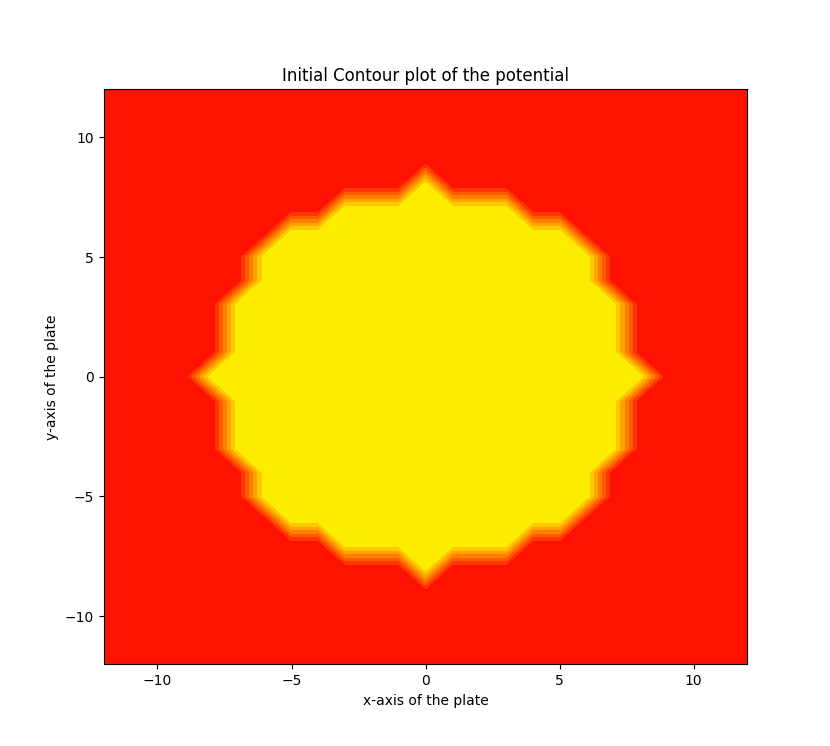
\includegraphics[height=8.5cm]{Figure_1.png}
\end{figure}

\textbf{cos(cos(x)) graph in range of $(-2\pi,4\pi)$}\\

\begin{figure}[h!]
\centering
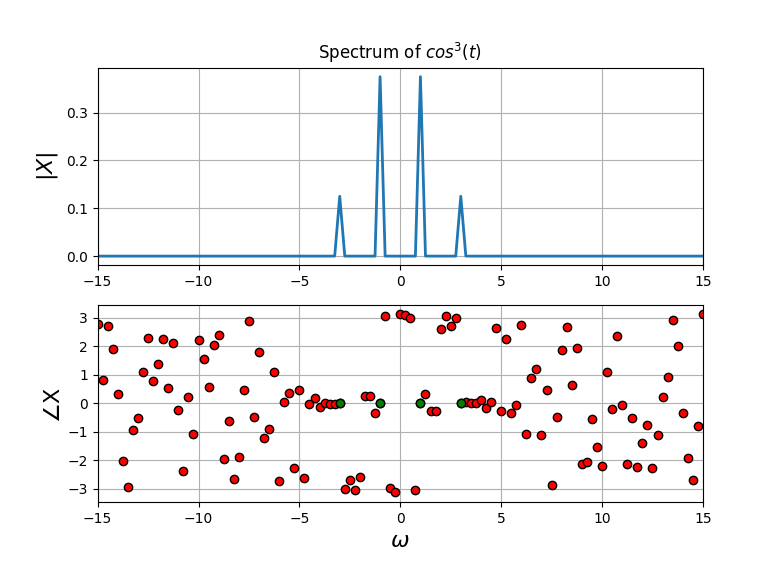
\includegraphics[height=8.5cm]{Figure_2.png}
\end{figure}

\newpage
As we see the graph, we can clearly notice that $e^x$ function is not periodic whereas cos(cos(x)) function is periodic with Time period=$\pi$.\\\\
\textbf{$e^x$ Approximation graph by Least Square Approch method and Integrate method:}
\begin{figure}[h!]
\centering
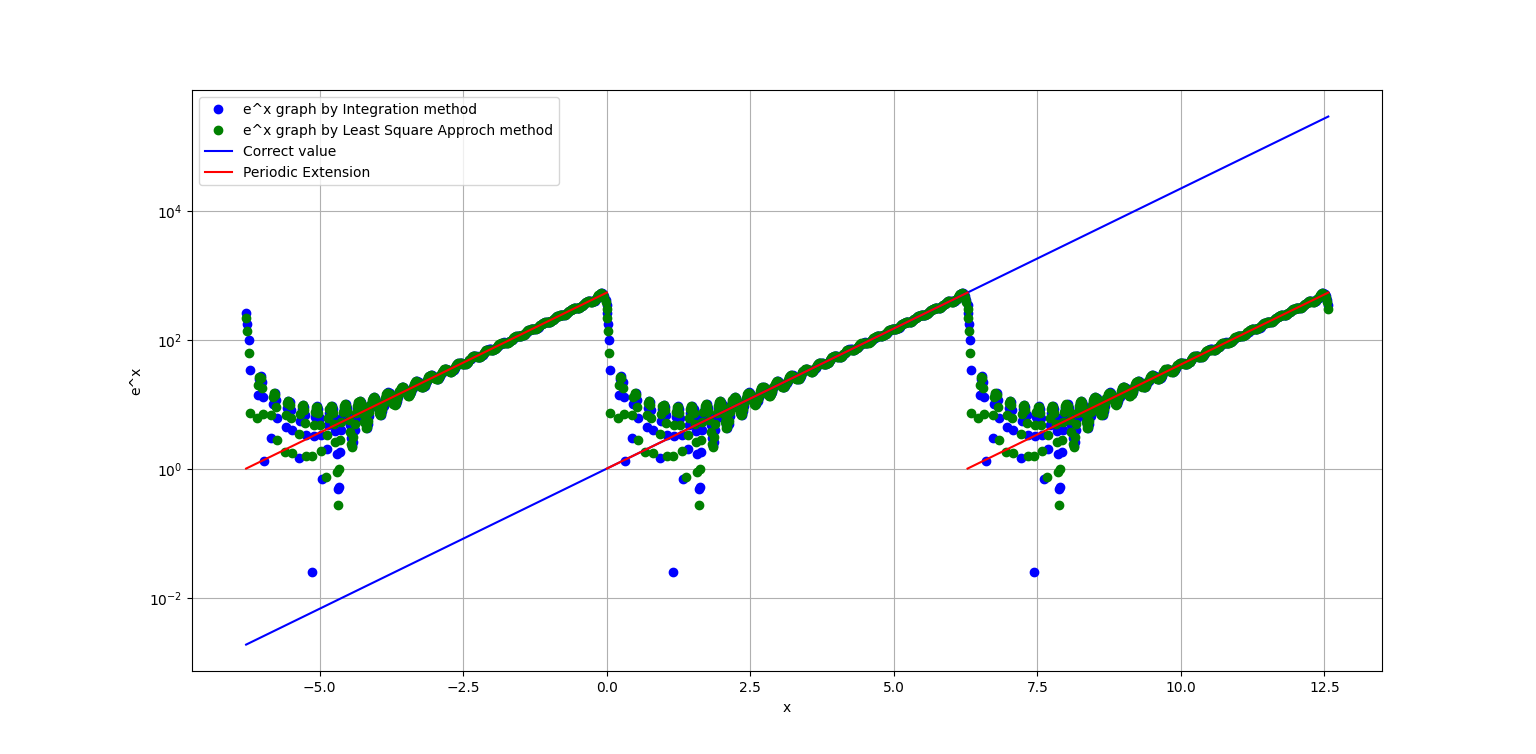
\includegraphics[height=10cm]{Figure_13.png}
\end{figure}

\section*{Question:6}
Maximum deviation of coefficients in $e^x$ function is 1.775420e+00\\
Maximum deviation of coefficients in cos(cos(x)) function is 2.643332e-15

\newpage
\section*{Question:3}

\textbf{A and B for $e^x$ function for Integration method in semilog graph.}

\begin{figure}[h!]
\centering
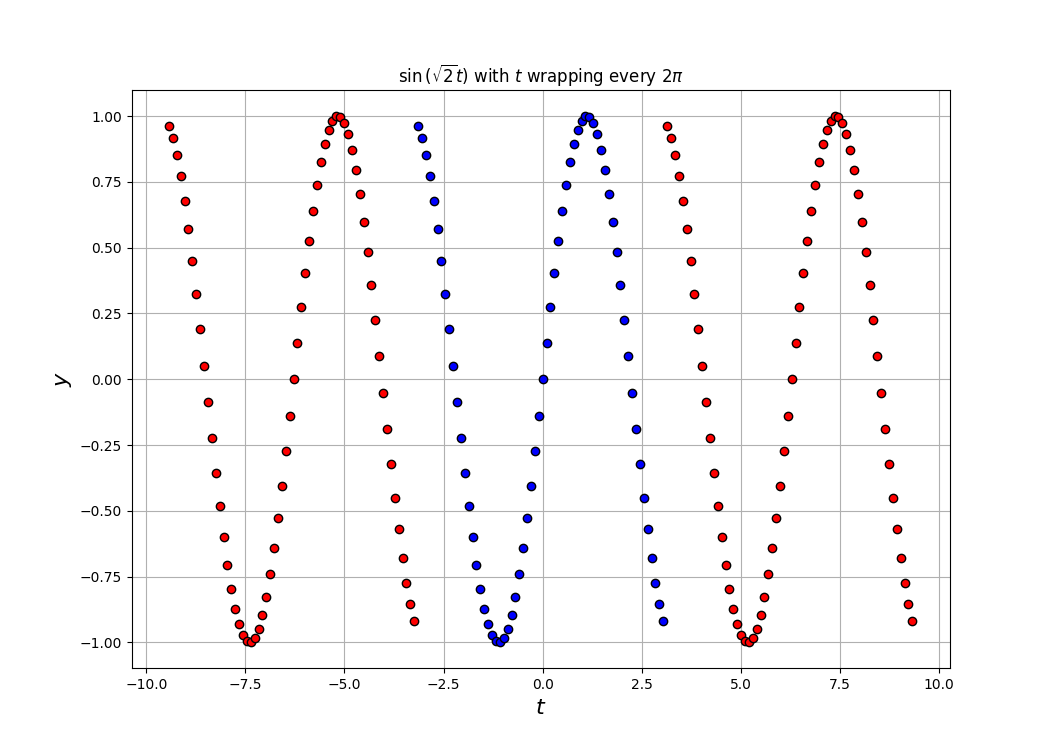
\includegraphics[height=8cm]{Figure_3.png}
\label{fig:exemplo}
\end{figure}

\textbf{A and B for $e^x$ function for Integration method in loglog graph.}

\begin{figure}[h!]
\centering
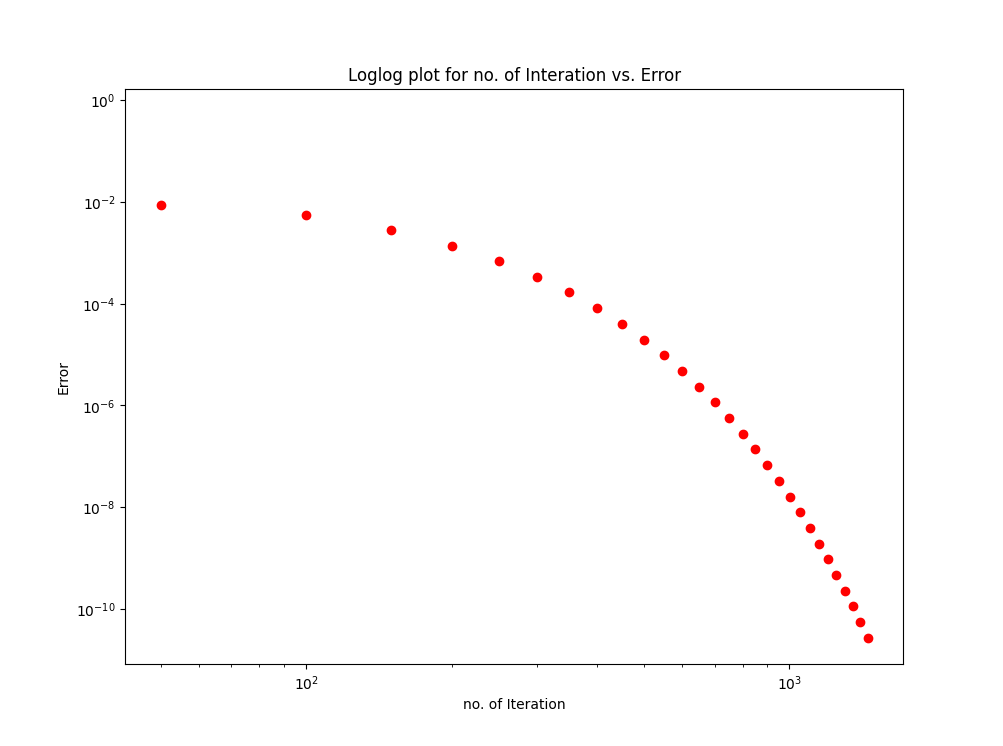
\includegraphics[height=8cm]{Figure_4.png}
\label{fig:exemplo}
\end{figure}
Inference: For $e^x$ function, both A and B coefficients decreases over n values, while magnitude of slope of A is more than of B.  
\newpage

\newpage
\textbf{A and B for cos(cos(x)) function for Integration method in semilog graph.}

\begin{figure}[h!]
\centering
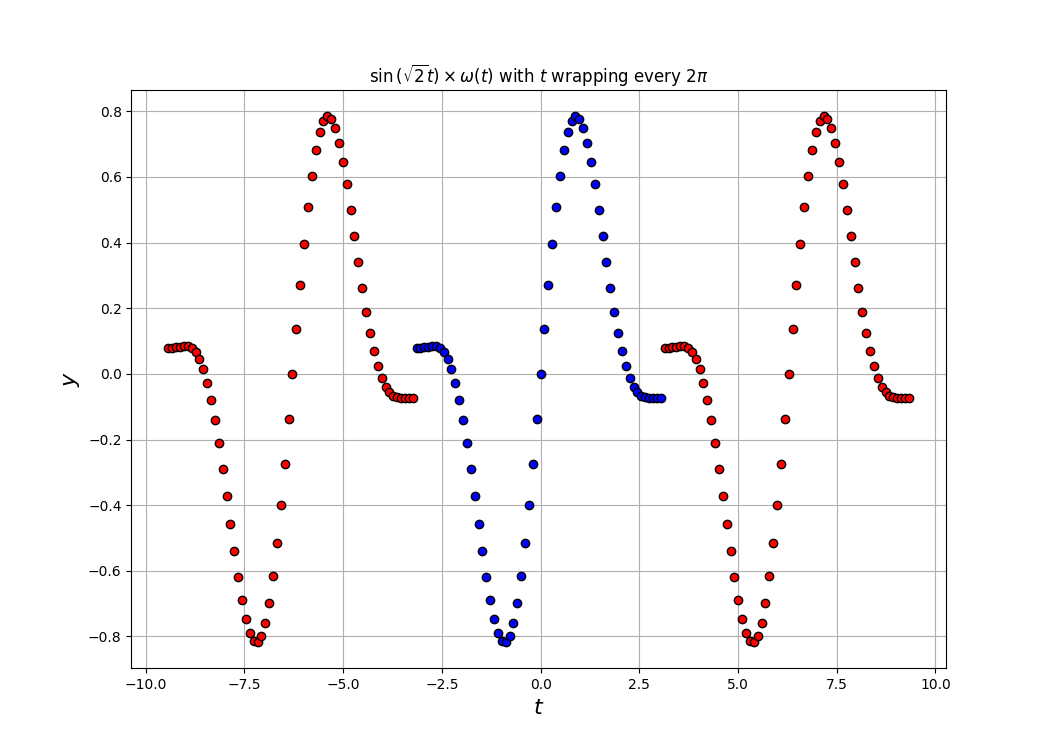
\includegraphics[height=8.5cm]{Figure_5.png}
\label{fig:exemplo}
\end{figure}

\textbf{A and B for cos(cos(x)) function for Integration method in loglog graph.}

\begin{figure}[h!]
\centering
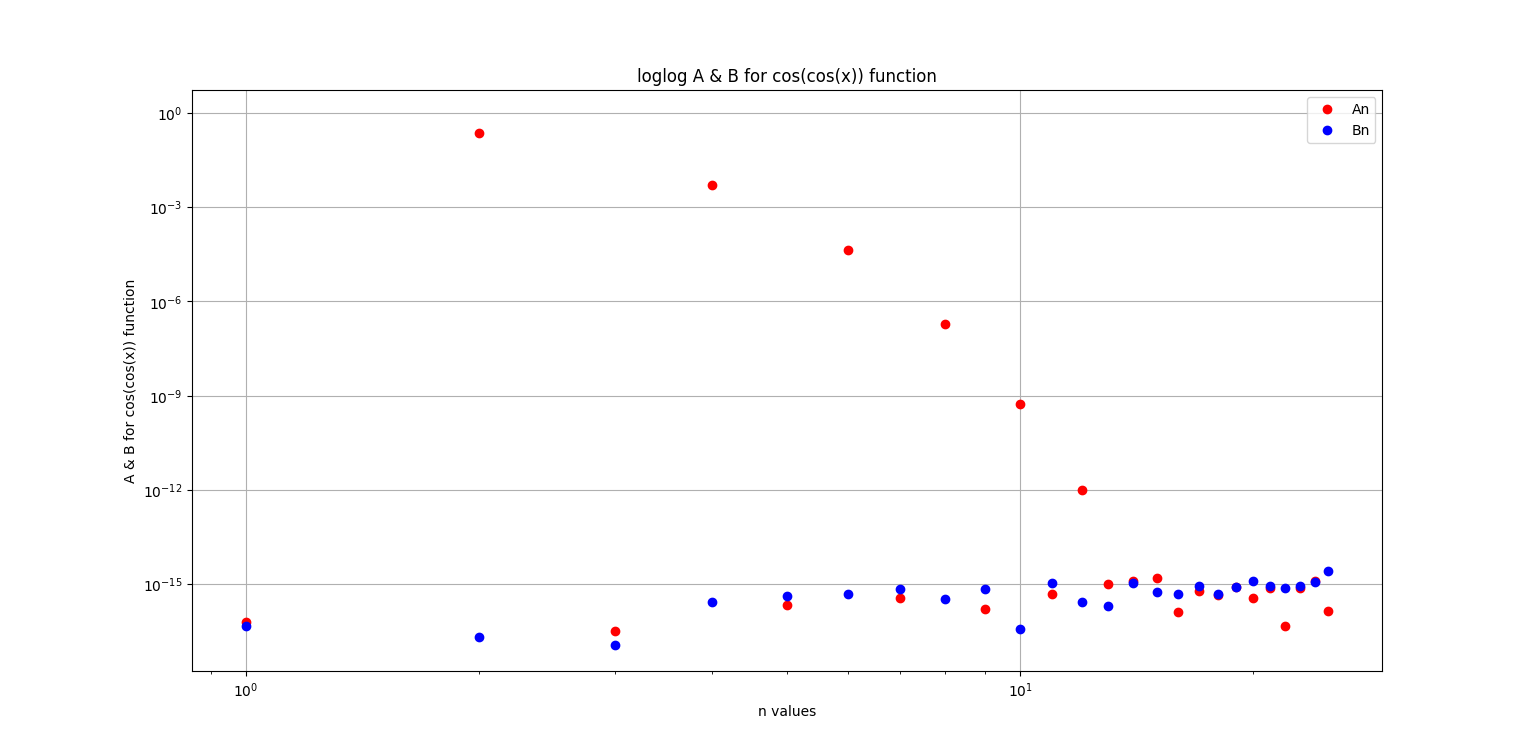
\includegraphics[height=8.5cm]{Figure_6.png}
\label{fig:exemplo}
\end{figure}
Inference: For cos(cos()) function, A coefficients vary more in the beginning and variation decreases over increase in n values, while B coefficients almost have same values.
\newpage
\section*{Question:4}

\textbf{Comparison of semilog graph A \& B in $e^x$ function in both methods.}\\\\
Here we can notice that the A coefficients obtained from both the methods vary more, whereas the B coefficients obtained from both the methods coincide each other without varying.

\begin{figure}[h!]
\centering
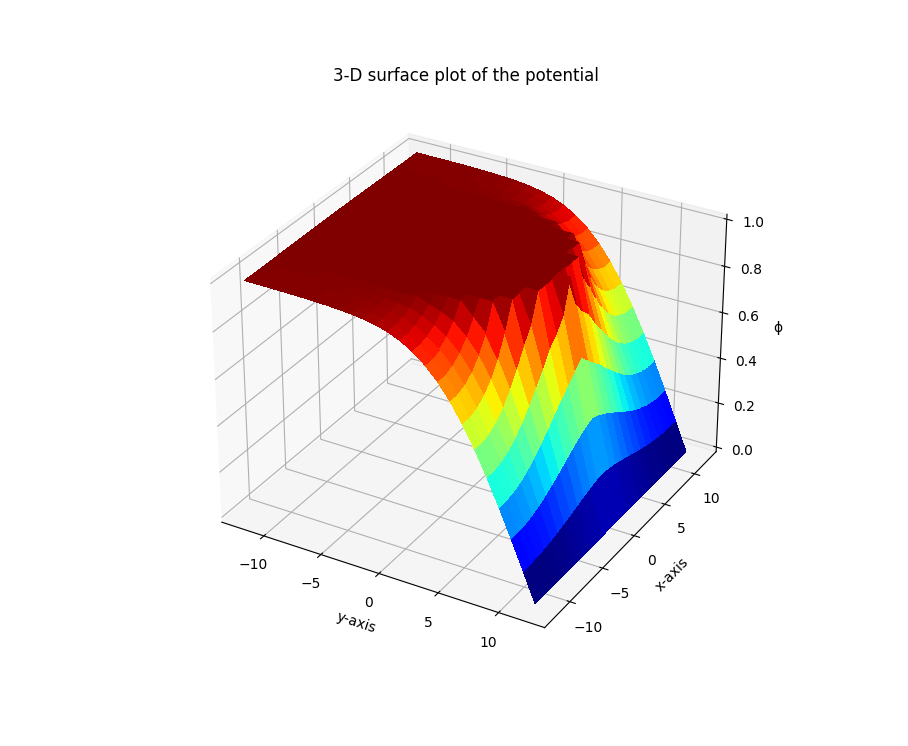
\includegraphics[height=6.8cm]{Figure_7.png}
\label{fig:exemplo}
\end{figure}

\textbf{Comparison of loglog graph A \& B in $e^x$ function in both methods.}\\\\
Here too we can notice the same pattern in above, Where A coefficients vary more and B coefficients coincide.

\begin{figure}[h!]
\centering
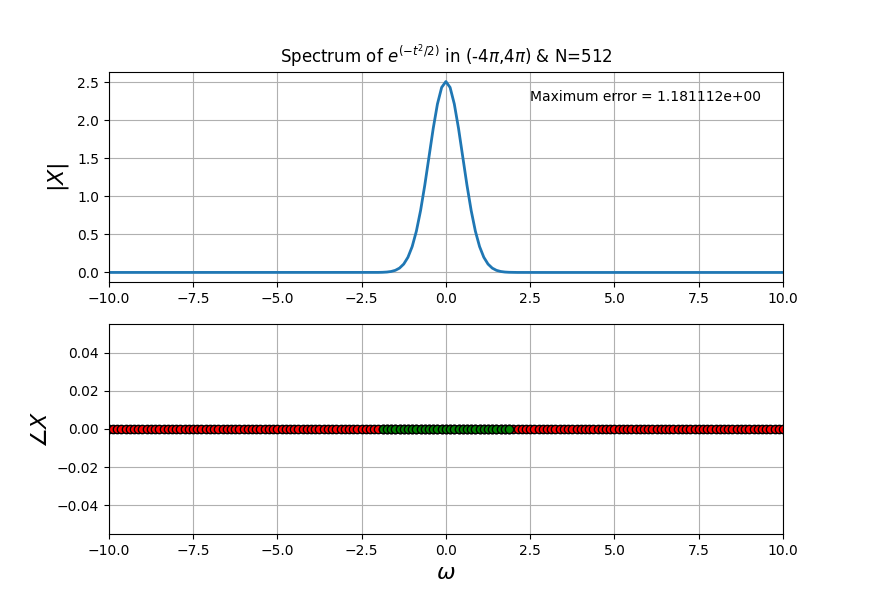
\includegraphics[height=6.8cm]{Figure_8.png}
\label{fig:exemplo}
\end{figure}
Inference: Thus for $e^x$ function, A varies more from both methods whereas B coincides.

\newpage
\textbf{Comparison of semilog A \& B in cos(cos(x)) function in both methods.}\\\\
Here we can notice that the A coefficients obtained from both the methods vary more in the beginning (Least squares approch method's A coefficient values are more than Integration method's A coefficient values) and variation decreases as n values increases.\\
Here B coefficients varies less (but doesn't coincide like in $e^x$ function).

\begin{figure}[h!]
\centering
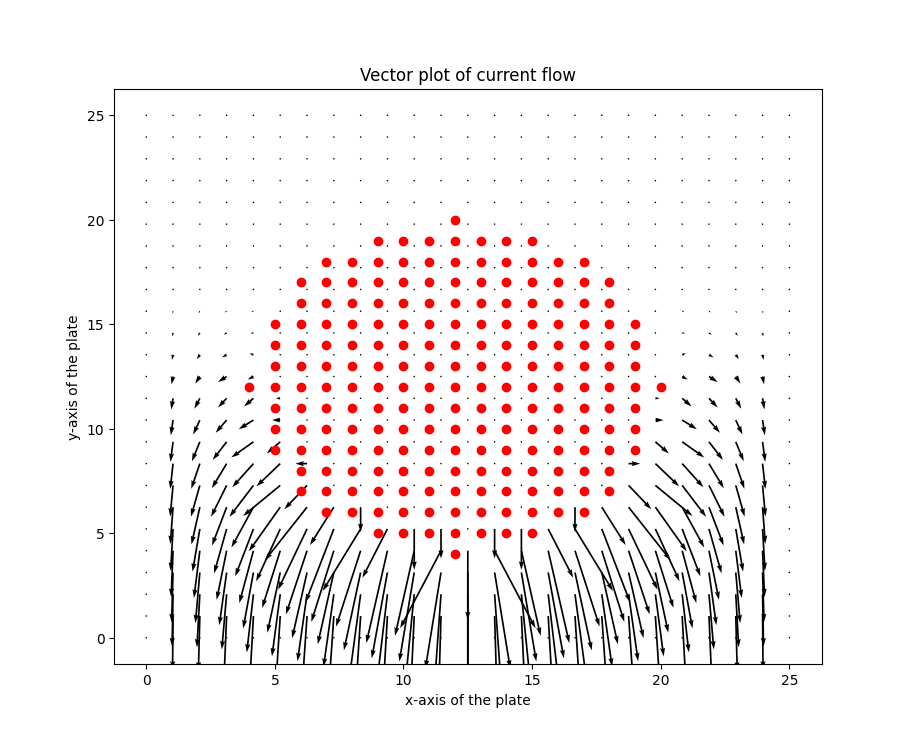
\includegraphics[height=7cm]{Figure_9.png}
\label{fig:exemplo}
\end{figure}

\textbf{Comparison of semilog A \& B in cos(cos(x)) function in both methods.}\\\\
Here too we can notice the same pattern as above, Where A coefficients vary more in beginning and then variation decrease as n value increases and B coefficients varies less.

\begin{figure}[h!]
\centering
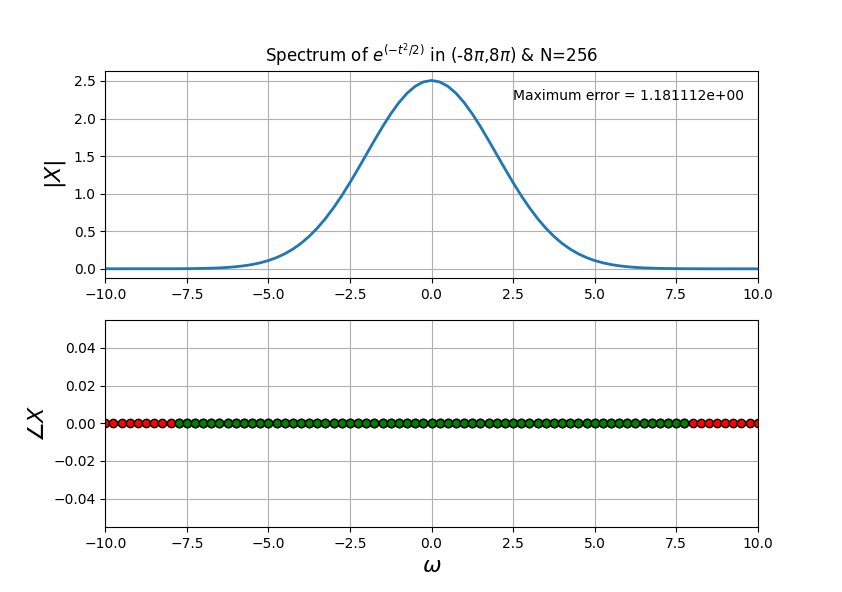
\includegraphics[height=7cm]{Figure_10.png}
\label{fig:exemplo}
\end{figure}

Inference: Thus for cos(cos(x)) function, A varies more in beginning and then variation decreases whereas B varies less throughout.


\newpage
\section*{Question:7}

\textbf{Comparison of Approximate $e^x$ graph optained with True function.}\\

\begin{figure}[h!]
\centering
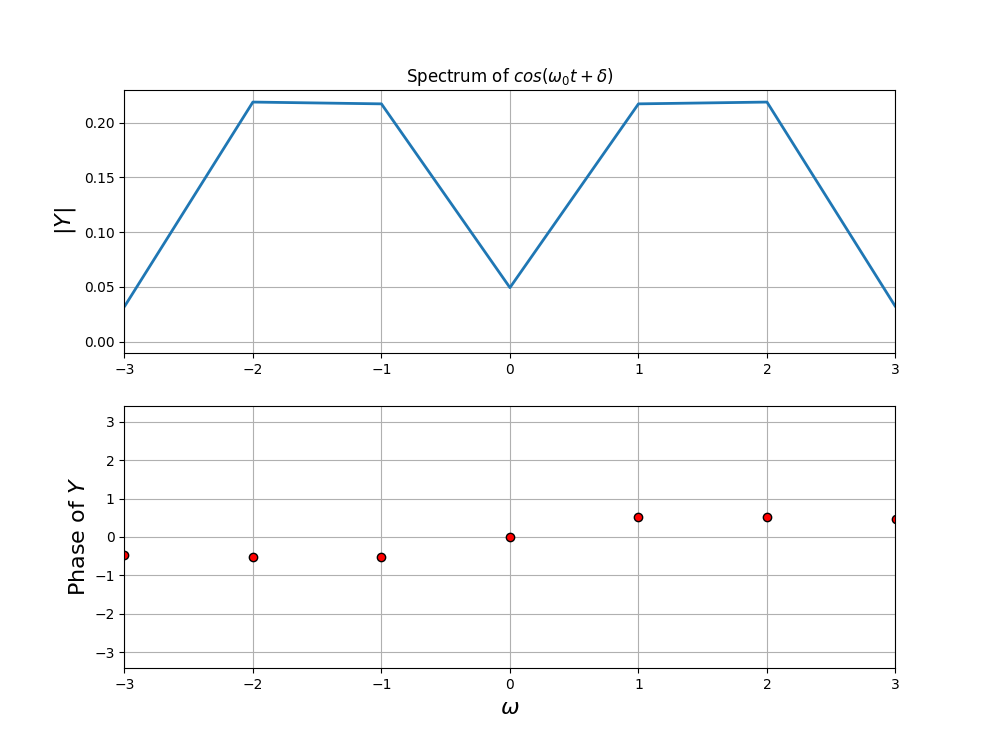
\includegraphics[height=8cm]{Figure_11.png}
\label{fig:exemplo}
\end{figure}

\textbf{Comparison of Approximate cos(cos(x)) graph optained with True function.}\\


\begin{figure}[h!]
\centering
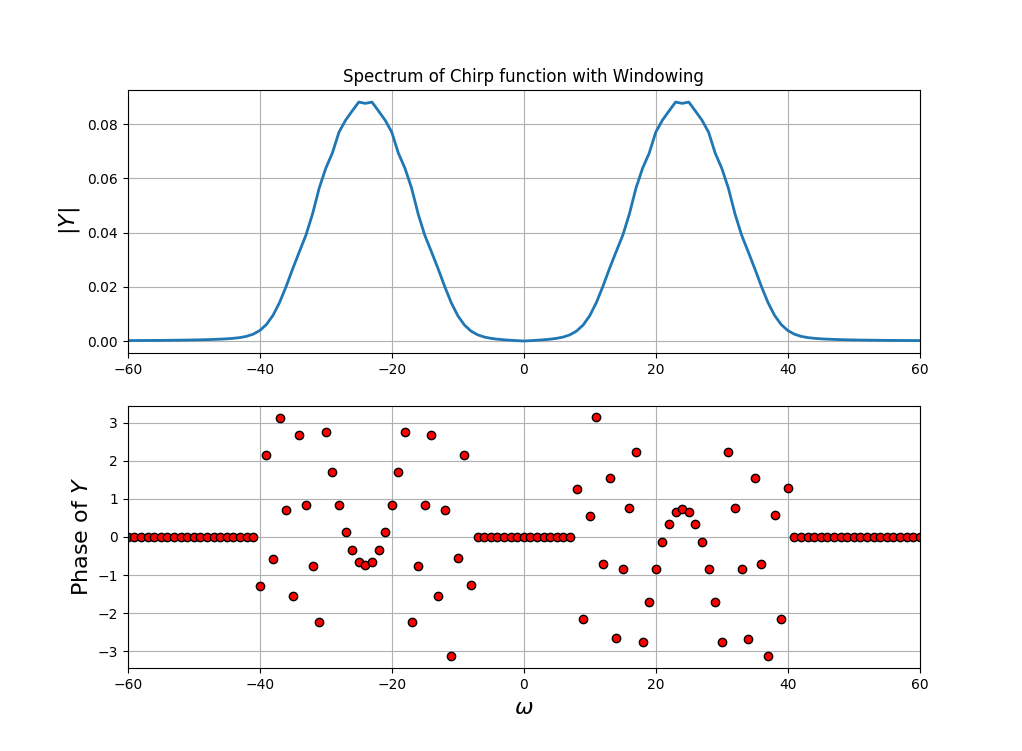
\includegraphics[height=8cm]{Figure_12.png}
\label{fig:exemplo}
\end{figure}
\begin{center} 
Thank you!
\end{center} 
\end{document}
